% DL-Project final report (draft). Build: latexmk -pdf report.tex
% All tables are generated by scripts/build_report_assets.py from C:\dlruns and \input below.
\documentclass[11pt,a4paper]{article}
\usepackage[margin=2.4cm]{geometry}
\usepackage[T1]{fontenc}
\IfFileExists{lmodern.sty}{\usepackage{lmodern}}{}
\usepackage{amsmath,amssymb}
\usepackage{booktabs}
\usepackage{graphicx}
\usepackage{caption}
\usepackage{xcolor}
\usepackage[numbers,sort&compress]{natbib}
\usepackage[hidelinks]{hyperref}
\usepackage{tabularx}
\usepackage{enumitem}
\setlist{nosep,leftmargin=1.4em}

\makeatletter\newcommand{\tabinput}[1]{\@@input #1 }\makeatother
\newcommand{\primary}{\textsc{primary}}
\newcommand{\exploratory}{\textsc{exploratory}}
\newcommand{\diagnostic}{\textsc{diagnostic}}
\newcommand{\reviewnote}[1]{\textcolor{red!70!black}{[\textbf{Review:} #1]}}

\title{Does Masked-Autoencoder Pretraining Improve Automatic Modulation Classification with Limited Labels?\\[0.3em]
\large A controlled comparison on RadioML 2018.01A}
\author{\reviewnote{author name, affiliation, course/module}}
\date{Draft, 21 October 2026}

\begin{document}
\maketitle

\begin{abstract}
We test whether self-supervised masked-autoencoder (MAE) pretraining of a patch-based 1-D convolutional encoder improves automatic modulation classification (AMC) on RadioML 2018.01A (24 classes, raw IQ input of shape $2\times1024$) when only part of the training labels is available.
The same classifier is fine-tuned either from random initialisation or from an MAE-pretrained encoder, using 1\%, 5\%, 10\%, 25\% and 100\% of the training labels, an identical optimisation recipe, validation-based checkpoint selection and a single evaluation on a held-out test set of 383,386 signals.
Across three seeds, the mean test macro-F1 of the MAE-initialised model was higher at 5\% labels (0.3320 vs.\ 0.3199; two of three seeds) and practically equal at 1\% (0.2566 vs.\ 0.2577) and 10\% (0.3571 vs.\ 0.3583).
Single-seed runs at 25\% and 100\% showed differences of $-0.0002$ and $+0.0017$.
No budget shows a consistent advantage that survives the observed seed-to-seed variation, so these experiments do not establish that MAE pretraining improves this classifier.
A follow-up diagnostic on the 5\% seed-42 runs found that BatchNorm running statistics are a substantial contributor to large epoch-to-epoch swings in validation metrics: exact recalibration of these statistics on the labelled training subset reduced the mean absolute epoch-to-epoch change in validation accuracy by 71--80\% and removed an epoch-7 dip in both arms.
We report this as a diagnostic finding that limits the precision of the primary comparison, not as a replacement result.
\end{abstract}

\section{Introduction}
Deep-learning AMC models are usually trained with abundant labels. Labels for radio signals can be costly to obtain in practice, which motivates representation learning from unlabelled IQ recordings. Masked autoencoders \citep{he2022mae} learn by reconstructing hidden parts of the input and have been effective for images; whether a comparable objective helps a small convolutional AMC model is an empirical question.

\paragraph{Research question.} \emph{For a fixed patch-based CNN classifier on RadioML 2018.01A \citep{oshea2018overtheair}, does initialising its encoder from MAE pretraining on the unlabelled training signals improve held-out classification performance relative to training from scratch, when 1\%, 5\%, 10\%, 25\% or 100\% of the training labels are available?}

\paragraph{Scope of this report.} The report describes a controlled comparison under one pre-specified protocol (Section~\ref{sec:protocol}), its primary results (Section~\ref{sec:results}), exploratory sensitivity checks performed after the primary test results were known (Section~\ref{sec:sensitivity}), and a diagnostic investigation of validation instability (Section~\ref{sec:bn}). Results are labelled \primary, \exploratory{} or \diagnostic{} throughout. We do not claim methodological novelty; the contribution is the controlled measurement and an honest account of its precision.

\section{Background}
\paragraph{Masked autoencoding.} An encoder sees only a random subset of input patches; a lightweight decoder reconstructs the hidden patches from the encoded visible ones and learned mask tokens, and the reconstruction loss is computed on the masked patches only \citep{he2022mae}. After pretraining the decoder is discarded and the encoder initialises a downstream model.

\paragraph{Batch normalisation.} During training a BatchNorm layer normalises each channel with statistics of the current mini-batch, and maintains running estimates for use at inference \citep{ioffe2015batchnorm}. In PyTorch these running estimates are exponential moving averages, $r \leftarrow (1-m)\,r + m\,b$ with momentum $m=0.1$, where $b$ is the batch mean or unbiased batch variance. With $m=0.1$ the last ten batches carry $1-0.9^{10}\approx 65\%$ of the weight, so the inference-time statistics depend on the final batches of an epoch.

\section{Data and protocol}\label{sec:protocol}

\subsection{Dataset and splits}
RadioML 2018.01A contains 2,555,904 IQ recordings of 1,024 complex samples (stored as $1024\times2$ float32), 24 modulation classes and 26 SNR levels from $-20$ to $+30$\,dB in 2\,dB steps.\footnote{Total size, class and SNR counts come from the project's dataset audit (\texttt{audit\_dataset.py}); the per-SNR keys of every result file confirm the 26 levels.}
A single split was fixed before any modelling: 70/15/15\% stratified by (class, SNR) with seed 42, giving 1,789,132 training, 383,386 validation and 383,386 test signals with disjoint index sets (\texttt{create\_splits.py}, \texttt{data\_splits.npz}).
No normalisation is fitted; both arms receive the raw IQ values, transposed to $2\times1024$.

\paragraph{Label budgets.} Class-balanced, nested labelled subsets were drawn from the training split once (seed 42; \texttt{create\_label\_subsets\_v2.py}): 17,883 (1\%), 89,451 (5\%), 178,914 (10\%), 447,281 (25\%) and 1,789,132 (100\%) signals. Every smaller subset is contained in every larger one.

\paragraph{Validation subset for checkpoint selection.} Classifier checkpoints are selected on a fixed subset of the validation split with 20 signals per (class, SNR) cell, i.e.\ $24\times26\times20 = 12{,}480$ signals (\texttt{create\_validation\_subset.py}, seed 42). The full validation split (383,386) is used only for selecting the MAE pretraining checkpoint.

\paragraph{Test set.} The 383,386 test signals were not used for training, hyperparameter choice or checkpoint selection in the primary protocol. Each selected checkpoint was evaluated on the test set once.

\subsection{Model}
The classifier (\texttt{src/models/cnn.py}) splits each $2\times1024$ signal into 16 non-overlapping patches of 64 samples. A shared encoder maps each patch to a 128-dimensional feature:
Conv1d($2\!\to\!32$, $k{=}7$, stride 2) -- BN -- GELU -- MaxPool(2) -- Conv1d($32\!\to\!64$, $k{=}5$) -- BN -- GELU -- MaxPool(2) -- Conv1d($64\!\to\!128$, $k{=}3$) -- BN -- GELU -- global average pool -- Linear($128\!\to\!128$).
Patch features are averaged over the 16 patches and a linear layer produces 24 logits. The classifier has 55,544 parameters (recorded in every test-result file), of which 52,448 belong to the encoder (derived from the layer definitions).
The encoder has no positional information across patches and averages patch features, so it cannot model the order of patches within a signal; we return to this in Section~\ref{sec:limitations}.

\subsection{MAE pretraining}
The MAE (\texttt{src/models/cnn\_mae.py}) uses the same encoder. For each signal, 8 of the 16 patches (mask ratio 0.5) are hidden at random; only the 8 visible patches are encoded. Learned positional embeddings are added, features are projected to the decoder width (128), mask tokens fill the hidden positions, and a 2-layer pre-norm Transformer decoder (4 heads, feed-forward width 512) followed by a linear head predicts the 128 values ($2\times64$) of every patch. With $\mathcal{M}$ the set of masked patches over a batch and $x_i,\hat{x}_i\in\mathbb{R}^{128}$ a target patch and its prediction, the loss is
\begin{equation}
\mathcal{L}_{\text{MAE}} = \frac{1}{|\mathcal{M}|}\sum_{i\in\mathcal{M}} \frac{1}{128}\,\lVert \hat{x}_i - x_i\rVert_2^2 .
\end{equation}
Pretraining used all 1,789,132 training signals without labels: AdamW (learning rate $10^{-4}$, weight decay $10^{-4}$), a per-epoch cosine schedule, batch size 64, gradient-norm clipping at 1.0, FP16 autocast, 5 epochs and seed 42 (\texttt{experiments/pretrain\_cnn\_mae\_fixed.py}). The checkpoint with the lowest validation MSE on the full validation split was kept.

\subsection{Fine-tuning (both arms)}
Both arms train the whole network with an identical recipe (\texttt{experiments/train\_classifier.py}): cross-entropy loss, AdamW (learning rate $10^{-3}$, weight decay $10^{-4}$), cosine annealing over 10 epochs stepped once per epoch, batch size 128, gradient-norm clipping at 1.0, FP16 autocast with gradient scaling, and no data augmentation. The \emph{only} difference is the encoder initialisation: random (scratch) or the weights of the selected MAE checkpoint (\texttt{cnn\_mae\_full\_v1\_best.pt}). The classification head is randomly initialised in both arms. After every epoch the model is evaluated on the 12,480-signal validation subset; the epoch with the highest validation macro-F1 is saved and is the only checkpoint evaluated on the test set.

Seeds 42, 43 and 44 were used at 1\%, 5\% and 10\%; seed 42 only at 25\% and 100\% (22 runs in total). The seed changes the head initialisation (and, for scratch, the encoder initialisation) and the mini-batch order; the label subsets and the MAE checkpoint are the same for all seeds. For speed, fine-tuning read the signals from bit-identical memory-mapped copies of the HDF5 data (\texttt{tools/build\_cache.py}, 300 spot checks per copy against the HDF5 file); the training code and recipe were unchanged.

\subsection{Metrics and statistics}
We report accuracy and macro-F1 over the 24 classes,
\begin{equation}
\text{macro-F1} = \frac{1}{24}\sum_{c=1}^{24} \frac{2\,\mathrm{TP}_c}{2\,\mathrm{TP}_c+\mathrm{FP}_c+\mathrm{FN}_c},
\end{equation}
together with accuracy per SNR, accuracy at SNR $\ge 10$\,dB, per-class F1 and confusion matrices (\texttt{experiments/evaluate\_test.py}). Macro-F1 is the headline metric because the test set is class-balanced and it weights every modulation equally.
For each budget and seed the two arms are compared on the same test signals with a paired bootstrap 95\% interval for the macro-F1 difference (1,000 resamples of test signals) and McNemar's test on per-signal correctness \citep{mcnemar1947} (\texttt{experiments/summarize\_results.py}). These quantify uncertainty from the finite test set \emph{for fixed trained models only}; they do not capture variation due to training randomness, which is the larger source of uncertainty here. Where three seeds exist we additionally give a paired $t$-statistic over seeds ($n=3$, 2 degrees of freedom), which is reported for completeness and has very little power.

\section{Primary results}\label{sec:results}

\subsection{MAE pretraining}
Table~\ref{tab:pretrain} lists the pretraining log. Validation MSE decreased in every epoch, so the final epoch (5) was selected (validation MSE 0.458528). Pretraining took 17,730\,s of wall-clock time.

A reconstruction check of the selected checkpoint (\texttt{tools/check\_mae.py}) on the validation subset gave a masked-patch MSE of 0.458, compared with 2.418 for predicting zeros and 0.497 for predicting each signal's mean over its visible patches. Relative to predicting zeros, the error ratio was about 1.0 at SNR $\le -10$\,dB and 0.07--0.09 at SNR $\ge 20$\,dB.
\reviewnote{These check\_mae figures are transcribed from the Phase-3 console output; the script prints and does not save them, so no stored file backs them. Re-run \texttt{tools/check\_mae.py} with output redirected to a file before submission, or remove this paragraph.}
Taken at face value, the encoder learned structure that is only recoverable at moderate and high SNR, and most of the zero-prediction error is explained by per-signal mean levels.

\begin{table}[htbp]
\centering\small
\caption{MAE pretraining (\texttt{C:\textbackslash dlruns\textbackslash cnn\_mae\_full\_v1.log}). Validation uses the full validation split (383,386 signals).}
\label{tab:pretrain}
\begin{tabular}{rccc}
\toprule
Epoch & Train MSE & Validation MSE & Learning rate used\\
\midrule
\tabinput{tables/pretraining.tex}
\bottomrule
\end{tabular}
\end{table}

\subsection{Scratch vs.\ MAE initialisation across label budgets (\primary)}
Table~\ref{tab:primary} and Figure~\ref{fig:label} give the test results of all 22 runs.

\begin{table}[htbp]
\centering\small
\caption{\primary{} test results (383,386 test signals). Means over seeds with sample standard deviation in parentheses; 25\% and 100\% are single runs (seed 42). $\Delta$ = MAE $-$ scratch macro-F1. ``Wins'' counts seeds with higher MAE macro-F1. Source: \texttt{C:\textbackslash dlruns\textbackslash results\textbackslash *\_v1.json}.}
\label{tab:primary}
\setlength{\tabcolsep}{4pt}
\begin{tabular}{lcccccccccc}
\toprule
 & & \multicolumn{2}{c}{Macro-F1} & & & \multicolumn{2}{c}{Accuracy} & \multicolumn{2}{c}{Acc.\ SNR$\ge$10\,dB}\\
\cmidrule(lr){3-4}\cmidrule(lr){7-8}\cmidrule(lr){9-10}
Labels & Seeds & Scratch & MAE & $\Delta$ & Wins & Scratch & MAE & Scratch & MAE\\
\midrule
\tabinput{tables/primary.tex}
\bottomrule
\end{tabular}
\end{table}

\begin{figure}[htbp]
\centering
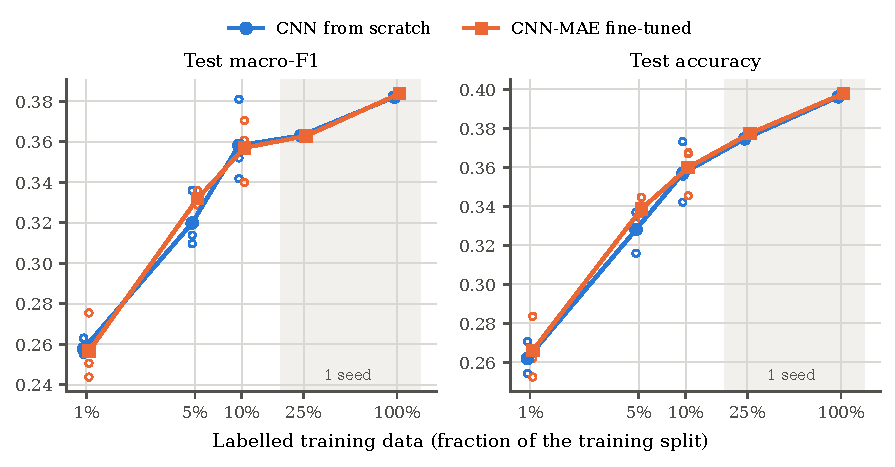
\includegraphics[width=\linewidth]{figures/fig_label_efficiency.pdf}
\caption{Test macro-F1 and accuracy against the labelled fraction (\primary). Lines: mean over seeds; hollow points: individual seeds. The shaded region marks budgets with a single seed.}
\label{fig:label}
\end{figure}

\paragraph{Observations.}
\begin{itemize}
\item \textbf{5\%:} the MAE arm had the higher mean macro-F1 ($+0.0121$; 0.3320 vs.\ 0.3199) and higher macro-F1 for seeds 42 and 43 but not 44. The per-seed differences were $+0.0219$, $+0.0191$ and $-0.0047$ (paired $t=1.43$, two-sided $p=0.29$, 2 d.f.).
\item \textbf{1\% and 10\%:} mean differences were $-0.0011$ and $-0.0012$, with one MAE win out of three seeds in each case, and per-seed differences of both signs ($+0.0124$ to $-0.0113$ at 1\%; $-0.0105$ to $+0.0087$ at 10\%).
\item \textbf{25\% and 100\% (single seed):} differences of $-0.0002$ and $+0.0017$. With one seed these are not estimates of a population-level effect; at 10\% the scratch seed-to-seed standard deviation alone was 0.0203.
\item \textbf{Accuracy} was slightly higher for the MAE arm at every budget (mean differences $+0.0041$, $+0.0106$, $+0.0031$, $+0.0028$, $+0.0017$), but again within the seed-to-seed variation except possibly at 5\%.
\item Performance rises steeply from 1\% to 10\% and then flattens: scratch macro-F1 increases by only 0.024 from 10\% to 100\% (single seed at 100\%).
\end{itemize}

\begin{table}[htbp]
\centering\small
\caption{Per-seed paired comparison on the test set (\primary). ``Epoch'' gives the validation-selected epoch for scratch / MAE. CI: paired bootstrap 95\% interval of the macro-F1 difference over test signals. $p$: McNemar test on per-signal correctness; values printed as 0 by the analysis script (below double-precision resolution) are shown as $<10^{-15}$. These intervals and $p$-values ignore training randomness. Source: \texttt{results\textbackslash paired\_comparison.csv}.}
\label{tab:perseed}
\setlength{\tabcolsep}{4pt}
\begin{tabular}{lcccccccc}
\toprule
Labels & Seed & Epoch & F1 scratch & F1 MAE & $\Delta$F1 & 95\% CI & $\Delta$Acc & $p$\\
\midrule
\tabinput{tables/per_seed.tex}
\bottomrule
\end{tabular}
\end{table}

\paragraph{Why the per-seed tests are not evidence of an effect.} Table~\ref{tab:perseed} shows that every per-seed interval but one (25\%) excludes zero, but with \emph{both signs}: at 1\% seed 42 favours MAE while seeds 43 and 44 favour scratch, each ``significantly''. With 383,386 test signals almost any difference between two trained networks is detectable, so these tests show that two particular models differ, not that the initialisation causes a reproducible difference. The relevant unit of replication is the training run, of which we have three per budget at most.

\subsection{Where the differences occur}
Figure~\ref{fig:snr} shows test accuracy by SNR. Both arms are at chance level ($\approx 1/24$) below about $-10$\,dB. At 1\% and 5\% the MAE arm is more accurate in the transition region: averaged over $-8$ to $0$\,dB the difference was $+0.026$ (1\%) and $+0.028$ (5\%), peaking at $+0.047$ ($-4$\,dB at 1\%, $-2$\,dB at 5\%). At SNR $\ge 10$\,dB the difference was $-0.004$ at 1\% and $+0.010$ at 5\%. At larger budgets the curves almost coincide. These are descriptive means over three seeds without an uncertainty estimate per SNR level.

Figure~\ref{fig:perclass} gives per-class F1 at 5\%. The largest differences were for 4ASK ($+0.107$ for MAE), AM-DSB-SC ($+0.056$) and 8PSK ($-0.055$). Many high-order QAM, APSK and PSK classes have F1 below 0.15 in both arms, which contributes to the gap between accuracy at SNR $\ge10$\,dB (0.49--0.50 at 5\%) and overall macro-F1.

\begin{figure}[htbp]
\centering
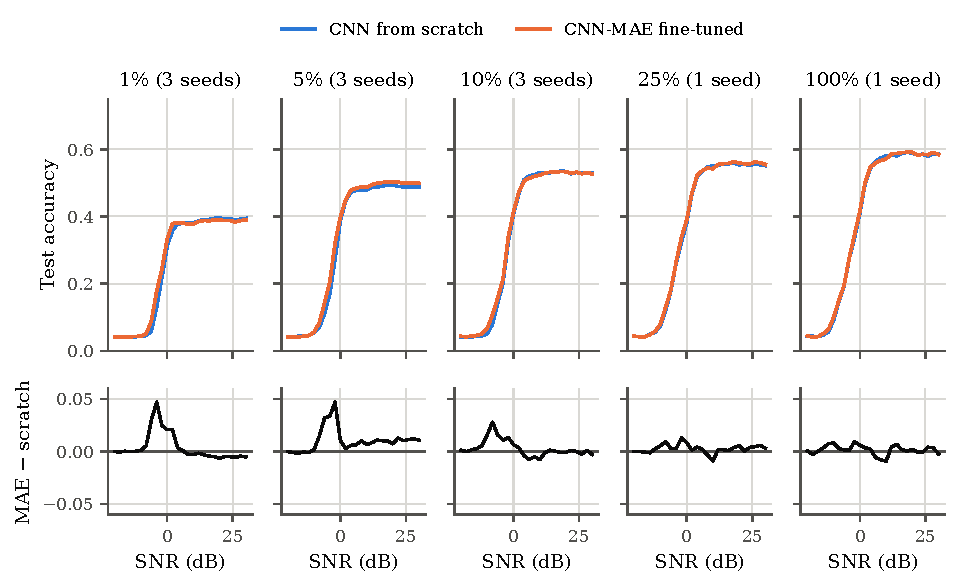
\includegraphics[width=\linewidth]{figures/fig_accuracy_vs_snr.pdf}
\caption{Test accuracy by SNR (top; mean over available seeds) and the MAE $-$ scratch difference (bottom). 25\% and 100\% are single runs.}
\label{fig:snr}
\end{figure}

\begin{figure}[htbp]
\centering
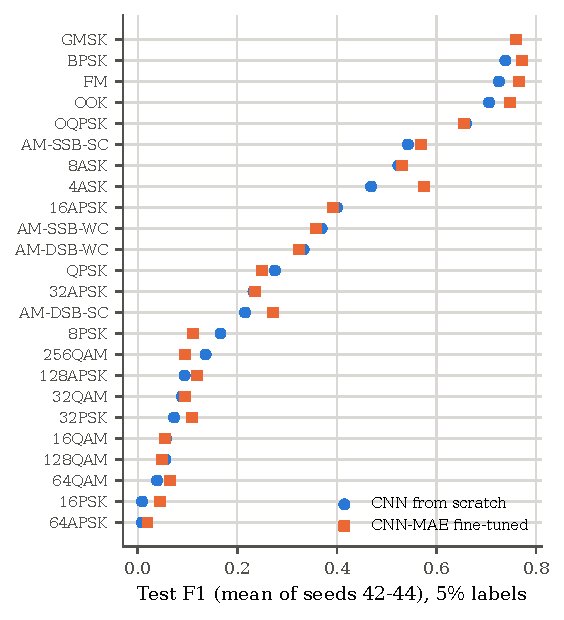
\includegraphics[width=0.55\linewidth]{figures/fig_per_class_f1_5pct.pdf}
\caption{Per-class test F1 at 5\% labels, mean of seeds 42--44 (\primary), sorted by the scratch arm.}
\label{fig:perclass}
\end{figure}

\section{Exploratory sensitivity analyses}\label{sec:sensitivity}
\emph{All analyses in this section were run after the primary test results had been observed} (primary test evaluation completed on 20 October around 21:05; the first sweep run began around 21:48, local time, from file timestamps in \texttt{C:\textbackslash dlruns}). They are therefore \exploratory{} and do not modify the primary protocol or results.

\subsection{Learning rate, weight decay and encoder learning rate (validation only)}
Table~\ref{tab:sens} and Figure~\ref{fig:sens} report the best validation macro-F1 at 5\% labels, seed 42; the test set was not used. The primary setting (learning rate $10^{-3}$) was best for both arms among the three learning rates; at $3\times10^{-4}$ the ordering of the arms reversed. Weight decay between $10^{-5}$ and $10^{-3}$ changed validation macro-F1 by at most 0.005 in either arm. Giving the pretrained encoder a lower learning rate than the head ($10^{-4}$ or $3\times10^{-4}$ vs.\ $10^{-3}$) gave 0.2448 and 0.2701, well below the 0.3385 obtained with equal rates under the same weight decay.
\reviewnote{The learning-rate sweep checkpoints do not record a weight-decay value; at that time the fine-tuning script used a fixed weight decay of $10^{-4}$, which is assumed here.}
Each point is a single run; given the epoch-to-epoch validation swings in Section~\ref{sec:bn}, differences below about 0.01--0.02 should not be interpreted.

\begin{table}[htbp]
\centering\small
\caption{\exploratory{} sweeps: best validation macro-F1 (12,480-signal validation subset), 5\% labels, seed 42. Rows marked ``primary'' reuse the primary runs. Sources: \texttt{finetune}, \texttt{tuning\_lr}, \texttt{tuning\_wd}, \texttt{tuning\_encoder\_lr} logs and checkpoint configs.}
\label{tab:sens}
\begin{tabular}{llcc}
\toprule
Setting & Value & Scratch & MAE\\
\midrule
\tabinput{tables/sensitivity.tex}
\bottomrule
\end{tabular}
\end{table}

\begin{figure}[htbp]
\centering
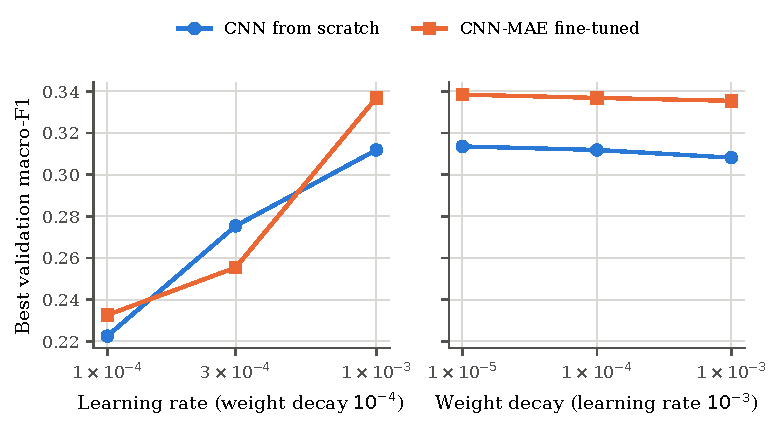
\includegraphics[width=0.75\linewidth]{figures/fig_sensitivity.pdf}
\caption{\exploratory{} learning-rate and weight-decay sweeps (validation only; 5\% labels, seed 42).}
\label{fig:sens}
\end{figure}

\subsection{Matched weight decay $10^{-5}$ at 5\%, seeds 42--44 (test set; exploratory)}
Because weight decay $10^{-5}$ was marginally best on validation, the 5\% comparison was repeated for all three seeds with that setting and evaluated on the test set (Table~\ref{tab:matched}). The mean macro-F1 was 0.3196 (scratch) vs.\ 0.3322 (MAE), a difference of $+0.0126$ with the same two-of-three seed pattern; mean accuracy was 0.3277 vs.\ 0.3389 and accuracy at SNR $\ge10$\,dB 0.4885 vs.\ 0.4989. Per seed, the test macro-F1 moved by at most 0.0018 relative to the primary runs. This shows that the 5\% result is insensitive to weight decay in this range; it is not independent evidence, since it reuses the same seeds, label subset and MAE checkpoint, and it was run after the test results were known. It is not merged with the primary results.

\begin{table}[htbp]
\centering\small
\caption{\exploratory{} test macro-F1 at 5\% labels with weight decay $10^{-5}$ (learning rate $10^{-3}$). Source: \texttt{C:\textbackslash dlruns\textbackslash results\_matched\_wd1e5\textbackslash test\_summary.csv}.}
\label{tab:matched}
\begin{tabular}{lccc}
\toprule
Seed & Scratch & MAE & MAE $-$ scratch\\
\midrule
\tabinput{tables/matched_wd1e5.tex}
\bottomrule
\end{tabular}
\end{table}

\section{Validation instability and BatchNorm statistics (diagnostic)}\label{sec:bn}
The training logs show validation metrics that rise and fall sharply between consecutive epochs while training loss decreases smoothly, in both arms and at the same epochs (for example, 5\% seed 42: validation macro-F1 0.3110 at epoch 6, 0.2670 at epoch 7 and 0.3086 at epoch 8 for scratch). These swings are larger than the MAE--scratch differences above, so we investigated them. All measurements in this section use the validation subset only; the test set was not used.

\subsection{Checkpoint-level diagnostic}
For the two 5\% seed-42 checkpoints (both selected at epoch 5) we evaluated the validation subset under four conditions (\texttt{tools/diag\_bn\_scratch\_5pct.py}, \texttt{tools/diag\_bn\_mae\_5pct.py}; Table~\ref{tab:bnckpt}):
(A) the original validation path, which reproduced the logged metrics exactly;
(A-FP32) the same without autocast;
(B) after exact recalibration of the BatchNorm running statistics on a copy of the model, using the 89,451 labelled training signals of the 5\% subset, computed layer by layer in evaluation mode with per-channel means and unbiased variances pooled over all samples and positions;
(C) 20 repetitions in which the running statistics were updated from 50 random training batches of 128 with PyTorch's own momentum rule, at fixed weights, which measures how much the batch sample alone moves the metrics.

\begin{table}[htbp]
\centering\small
\caption{\diagnostic{} checkpoint-level validation results (accuracy / macro-F1), 5\% labels, seed 42, epoch 5. C: range over 20 draws. Source: \texttt{C:\textbackslash dlruns\textbackslash diagnostics\textbackslash bn\_\{scratch,mae\}\_5pct\_seed42\textbackslash results.json}.}
\label{tab:bnckpt}
\footnotesize\setlength{\tabcolsep}{3pt}
\begin{tabular}{lccccc}
\toprule
Arm & A (as logged) & A-FP32 & B (recalibrated) & C accuracy & C macro-F1\\
\midrule
\tabinput{tables/bn_checkpoint.tex}
\bottomrule
\end{tabular}
\end{table}

FP16 autocast changed accuracy by less than 0.001. Recalibration raised validation accuracy by 0.038 (scratch) and 0.032 (MAE); macro-F1 rose by 0.020 for scratch but fell by 0.006 for MAE. The change was concentrated in the last BatchNorm layer, whose stored running variance exceeded the recalibrated variance (median ratio of recalibrated to stored variance 0.685 and 0.663). Updating only the running statistics from random training batches at fixed weights moved validation accuracy over 0.270--0.341 (scratch) and 0.281--0.348 (MAE); the selected checkpoints lay at the 85th and 80th percentiles of these draws. The validation metrics are therefore highly sensitive to the stored statistics. This alone does not show that the statistics caused the swings during training.

\subsection{Per-epoch diagnostic}
To test the training trajectory directly, the original 5\% seed-42 fine-tuning was rerun for each arm with the unmodified training code, adding after every epoch an evaluation of a recalibrated \emph{copy} of the model (\texttt{tools/diag\_perepoch\_5pct.py}).
The copy never affected training: model, optimiser, scheduler and gradient-scaler states were compared before and after every measurement, random-number states were restored, and the reruns reproduced the original logs at printed precision for all ten epochs, selected epoch 5 again, and produced epoch-5 weights and selected checkpoints bitwise identical to the originals. Ordinary validation therefore refers to the same numbers as the original runs, and checkpoint selection was unchanged.

Analysis criteria were fixed before the runs: over epochs 4--10, a dip is a drop of more than 0.03 from the previous epoch (separately for accuracy and macro-F1), and recalibration is said to remove the instability if the recalibrated mean absolute epoch-to-epoch change is at most half the ordinary one and no ordinary dip recurs in the recalibrated series.

\begin{table}[htbp]
\centering\small
\caption{\diagnostic{} per-epoch validation stability over epochs 4--10 (5\% labels, seed 42). Mean $|\Delta|$: mean absolute change between consecutive epochs. Source: \texttt{C:\textbackslash dlruns\textbackslash diagnostics\textbackslash perepoch\_5pct\_seed42\textbackslash \{scratch,mae\}\textbackslash summary.json}.}
\label{tab:bnpe}
\setlength{\tabcolsep}{4pt}
\begin{tabular}{llcccccc}
\toprule
 & & \multicolumn{2}{c}{Mean $|\Delta|$} & \multicolumn{2}{c}{Range} & \multicolumn{2}{c}{Dip epochs}\\
\cmidrule(lr){3-4}\cmidrule(lr){5-6}\cmidrule(lr){7-8}
Arm & Metric & Ordinary & Recal. & Ordinary & Recal. & Ordinary & Recal.\\
\midrule
\tabinput{tables/bn_perepoch.tex}
\bottomrule
\end{tabular}
\end{table}

\begin{figure}[htbp]
\centering
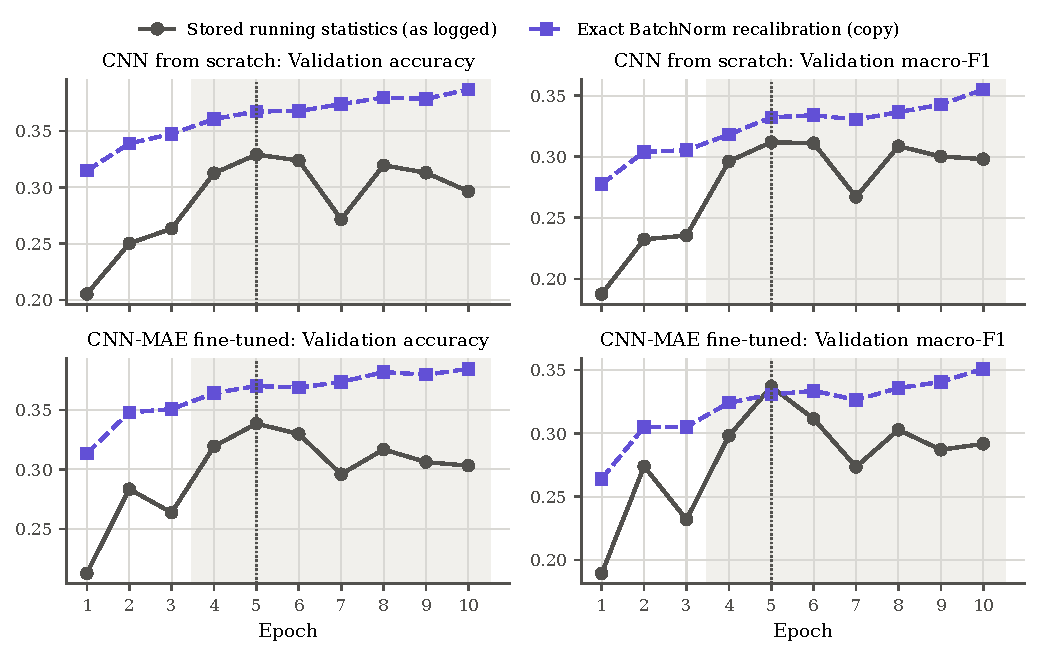
\includegraphics[width=\linewidth]{figures/fig_bn_perepoch.pdf}
\caption{\diagnostic{} validation metrics per epoch with the stored running statistics (as logged) and after exact recalibration of a model copy, 5\% labels, seed 42. Dotted line: epoch selected by the primary protocol; shaded: analysis window.}
\label{fig:bnpe}
\end{figure}

Table~\ref{tab:bnpe} and Figure~\ref{fig:bnpe} show the results. In both arms recalibration reduced the mean absolute epoch-to-epoch change in accuracy from 0.0242 to 0.0048 (scratch) and from 0.0160 to 0.0046 (MAE), and in macro-F1 from 0.0188 to 0.0073 and from 0.0254 to 0.0069; the epoch-7 dip present in both metrics and both arms disappeared, so the pre-specified criterion was met in all four cases. The relative change in weights between epochs decreased steadily (scratch: 0.205 at epoch 2 to 0.004 at epoch 10; 0.038 at epoch 7), so the epoch-7 dip did not coincide with a large weight update.

Two further observations are reported for completeness. Under recalibration both curves increased almost monotonically and reached their maxima at epoch 10 (macro-F1 0.3550 scratch, 0.3510 MAE), whereas the protocol selected epoch 5. And the MAE $-$ scratch difference in recalibrated validation macro-F1 stayed within $-0.004$ to $+0.006$ for epochs 2--10, compared with $-0.013$ to $+0.042$ under the stored statistics; the $+0.025$ validation advantage of the MAE arm at the selected epoch is not present after recalibration in this seed.

\subsection{Interpretation}
For the two runs examined, BatchNorm running statistics are a substantial contributor to the epoch-to-epoch validation instability: removing their sampling noise, with weights unchanged, eliminated the largest dip and reduced the mean absolute epoch-to-epoch change by 61--80\% across the two arms and two metrics. This does not show that all instability is explained, that the same holds for other seeds or budgets, or that test performance would change. The recalibrated metrics are diagnostic measurements on the validation subset and do not replace the primary protocol.

The finding matters for the primary comparison in two ways. First, checkpoint selection on validation metrics that move by several points with the BatchNorm state is noisy, and the selected checkpoints were near the top of the range attainable by resampling the statistics, so selected validation scores are likely optimistic. Second, the test evaluation uses the same stored statistics, so per-seed test differences of 0.01--0.02 between arms are of the same order as variation that can be produced by the BatchNorm state alone. The primary per-seed differences should be read with this in mind; we did not evaluate recalibrated models on the test set.

\section{Discussion}
\paragraph{Answer to the research question.} Under this protocol, MAE pretraining of this encoder did not produce a consistent improvement. Among the budgets with three seeds, only 5\% shows a higher mean macro-F1 for the MAE arm; there two of three seeds favour MAE and the across-seed evidence is weak ($p=0.29$ with three seeds); at 1\% and 10\% the arms are indistinguishable, and the 25\% and 100\% comparisons rest on one seed each. In the one diagnostic setting examined (5\%, seed 42), the validation advantage of the MAE arm disappeared once BatchNorm statistics were recalibrated.

\paragraph{Possible explanations (not tested).} The MAE appears to have learned reconstructable structure mainly at moderate to high SNR, and its error is close to that of a per-signal mean predictor overall, which leaves limited room for transferable features. The encoder sees each 64-sample patch independently and the classifier averages patch features; both the reconstruction task and the classifier are therefore restricted to within-patch structure. Fine-tuning the whole network at learning rate $10^{-3}$ may also overwrite much of the pretrained initialisation, although the lower encoder learning rates that were tried performed worse. The modest gains concentrated in the $-8$ to $0$\,dB region at 1\% and 5\% are consistent with the pretrained encoder providing some robustness in the low-SNR transition region, but this was not tested statistically.

\section{Limitations}\label{sec:limitations}
\begin{itemize}
\item \textbf{Seeds.} Three seeds at 1/5/10\% and one at 25/100\%. Seed-to-seed standard deviations (up to 0.020 macro-F1) exceed most of the measured differences. Label subsets and the MAE checkpoint were fixed across seeds, so their variability is not represented.
\item \textbf{Single MAE run.} One pretraining run (5 epochs, mask ratio 0.5, one architecture) was used; no alternative pretraining settings were compared.
\item \textbf{Model capacity.} The patch-wise encoder with mean pooling reaches 0.382 macro-F1 and 0.585 accuracy at SNR $\ge10$\,dB with all labels, so conclusions apply to this architecture, not to AMC models in general.
\item \textbf{Validation-based selection with unstable BatchNorm statistics} (Section~\ref{sec:bn}); the diagnostic covers one budget and one seed per arm.
\item \textbf{Exploratory analyses after test exposure.} The sweeps and the matched weight-decay test evaluation were run after the primary test results were known.
\item \textbf{Compute is not equalised.} The MAE arm received an additional 17,730\,s of pretraining on the unlabelled training signals; wall-clock fine-tuning times were measured on a shared workstation without controlling for other load.
\item \textbf{Unlabelled data.} Pretraining used all training signals of the same distribution; results may differ with unlabelled data from other conditions.
\end{itemize}

\section{Future work}
\begin{itemize}
\item Repeat the comparison with more seeds per budget, including resampled label subsets and independent MAE pretraining runs, so that the across-run variance can be estimated.
\item Make the validation protocol robust to BatchNorm sampling noise, for example by recalibrating BatchNorm statistics before each validation pass, and pre-register that change before any new test evaluation; or compare with normalisation layers that do not keep running statistics.
\item Evaluate encoders that model cross-patch structure (e.g.\ positional information and attention over patches), for which masked reconstruction may be a stronger pretext task.
\item Test whether the low-SNR gains at small budgets are reproducible with per-SNR confidence intervals.
\end{itemize}

\section{Reproducibility}\label{sec:repro}
\paragraph{Environment.} Python 3.11.9; PyTorch 2.10.0+cu126 and GPU ``NVIDIA GeForce RTX 4050 Laptop GPU'' (both recorded in the diagnostic result files); NumPy 2.4.6, h5py 3.16.0, scikit-learn 1.9.1 and matplotlib 3.11.2 in the virtual environment \texttt{C:\textbackslash venvs\textbackslash dlproj}.
\reviewnote{Library versions other than PyTorch come from the installation transcript, not from a stored file; CPU and RAM were not recorded. Export \texttt{pip freeze} to the report folder.}
GPU non-determinism was not disabled; nevertheless the two per-epoch reruns reproduced the original 5\% seed-42 runs bit for bit.

\paragraph{Cost.} MAE pretraining: 17,730\,s. Fine-tuning wall-clock (from logs): about 16--32\,s per run at 1\%, 63--138\,s at 5\%, 160--311\,s at 10\%, 517\,s (MAE) and 725\,s (scratch) at 25\%, and 9,289\,s (MAE) and 6,899\,s (scratch) at 100\%. Test inference ran at a median of about 50,000 signals/s (FP16, batch 1024, including data loading from the memory-mapped copy).

{\raggedright\paragraph{Artifacts.} All under \texttt{C:\textbackslash dlruns}:
\begin{itemize}
\item primary checkpoints and training logs: \texttt{finetune};
\item primary test outputs (per-run JSON, predictions, summaries): \texttt{results};
\item exploratory runs: \texttt{tuning\_lr}, \texttt{tuning\_wd}, \texttt{tuning\_encoder\_lr}, \texttt{matched\_wd1e5}, \texttt{results\_matched\_wd1e5};
\item diagnostics: \texttt{diagnostics}.
\end{itemize}
All figures and tables in this report are regenerated from these files by \texttt{report/scripts/build\_report\_assets.py}; \texttt{report/evidence\_map.md} links every reported number to its source.\par}

\paragraph{Result register.}
\begin{center}\small
\begin{tabularx}{\linewidth}{lX}
\toprule
\primary & 22 runs: scratch and MAE at 1/5/10\% (seeds 42--44) and 25/100\% (seed 42); learning rate $10^{-3}$, weight decay $10^{-4}$; one test evaluation each (Tables~\ref{tab:primary}--\ref{tab:perseed}, Figures~\ref{fig:label}--\ref{fig:perclass}).\\
\exploratory & Learning-rate, weight-decay and encoder-learning-rate sweeps (validation only); matched weight decay $10^{-5}$ test evaluation at 5\% (Section~\ref{sec:sensitivity}).\\
\diagnostic & BatchNorm checkpoint and per-epoch diagnostics, 5\% seed 42, validation only (Section~\ref{sec:bn}).\\
\bottomrule
\end{tabularx}
\end{center}

\bibliographystyle{plainnat}
\bibliography{references}
\end{document}
